\documentclass{beamer}
\usepackage{listings}
\lstset{
%language=C,
frame=single, 
breaklines=true,
columns=fullflexible
}
\usepackage{subcaption}
\usepackage{url}
\usepackage{tikz}
\usepackage{tkz-euclide} % loads  TikZ and tkz-base
%\usetkzobj{all}
\usetikzlibrary{calc,math}
\usepackage{float}
\newcommand\norm[1]{\left\lVert#1\right\rVert}
\renewcommand{\vec}[1]{\mathbf{#1}}
\usepackage[export]{adjustbox}
\usepackage[utf8]{inputenc}
\usepackage{amsmath}
\usetheme{Boadilla}
\usepackage{mathalfa}


\title{SNR Coverage Probability Analysis of RIS-Aided Communication Systems}
\author{Tanay Yadav - AI20BTECH11026}
\date{\today}
\begin{document}
\begin{frame}
\titlepage
\end{frame}
\section{Important Terminology}
\begin{frame}
    \frametitle{Important Terminology}
    \begin{block}{Re-configurable Intelligent Surface (RIS)}
        A re-configurable intelligent surface (RIS) is a two-dimensional surface of engineered material whose properties are re-configurable rather than static. The scattering, absorption, reflection, and diffraction properties can be changed with time and controlled by software.
    \end{block}
    \begin{block}{Coverage Probability}
        The coverage probability of a technique for calculating a confidence interval is the proportion of the time that the interval contains the true value of interest
    \end{block}
    \begin{block}{Fading Channel}
        A fading channel is a communication channel that experiences fading, i.e. variation of the attenuation of a signal with various variables
    \end{block}
\end{frame}
\begin{frame}
    \frametitle{Important Terminology}
    \begin{block}{Rayleigh Fading}
        Rayleigh fading is a statistical model for the effect of a propagation environment on a radio signal, such as that used by wireless devices.
    \end{block}
    \begin{block}{Signal to Noise ratio (SNR)}
        Signal-to-noise ratio is a measure used in science and engineering that compares the level of a desired signal to the level of background noise. SNR is defined as the ratio of signal power to the noise power, often expressed in decibels.
    \end{block}
    \begin{block}{TS and SR links}
        TS Link: Link between the signal transmitter and the RIS.
      \\SR Link: Link between the RIS and the signal receiver. 
    \end{block}
\end{frame}
\begin{frame}{System Model}
    \begin{figure}
        \centering
        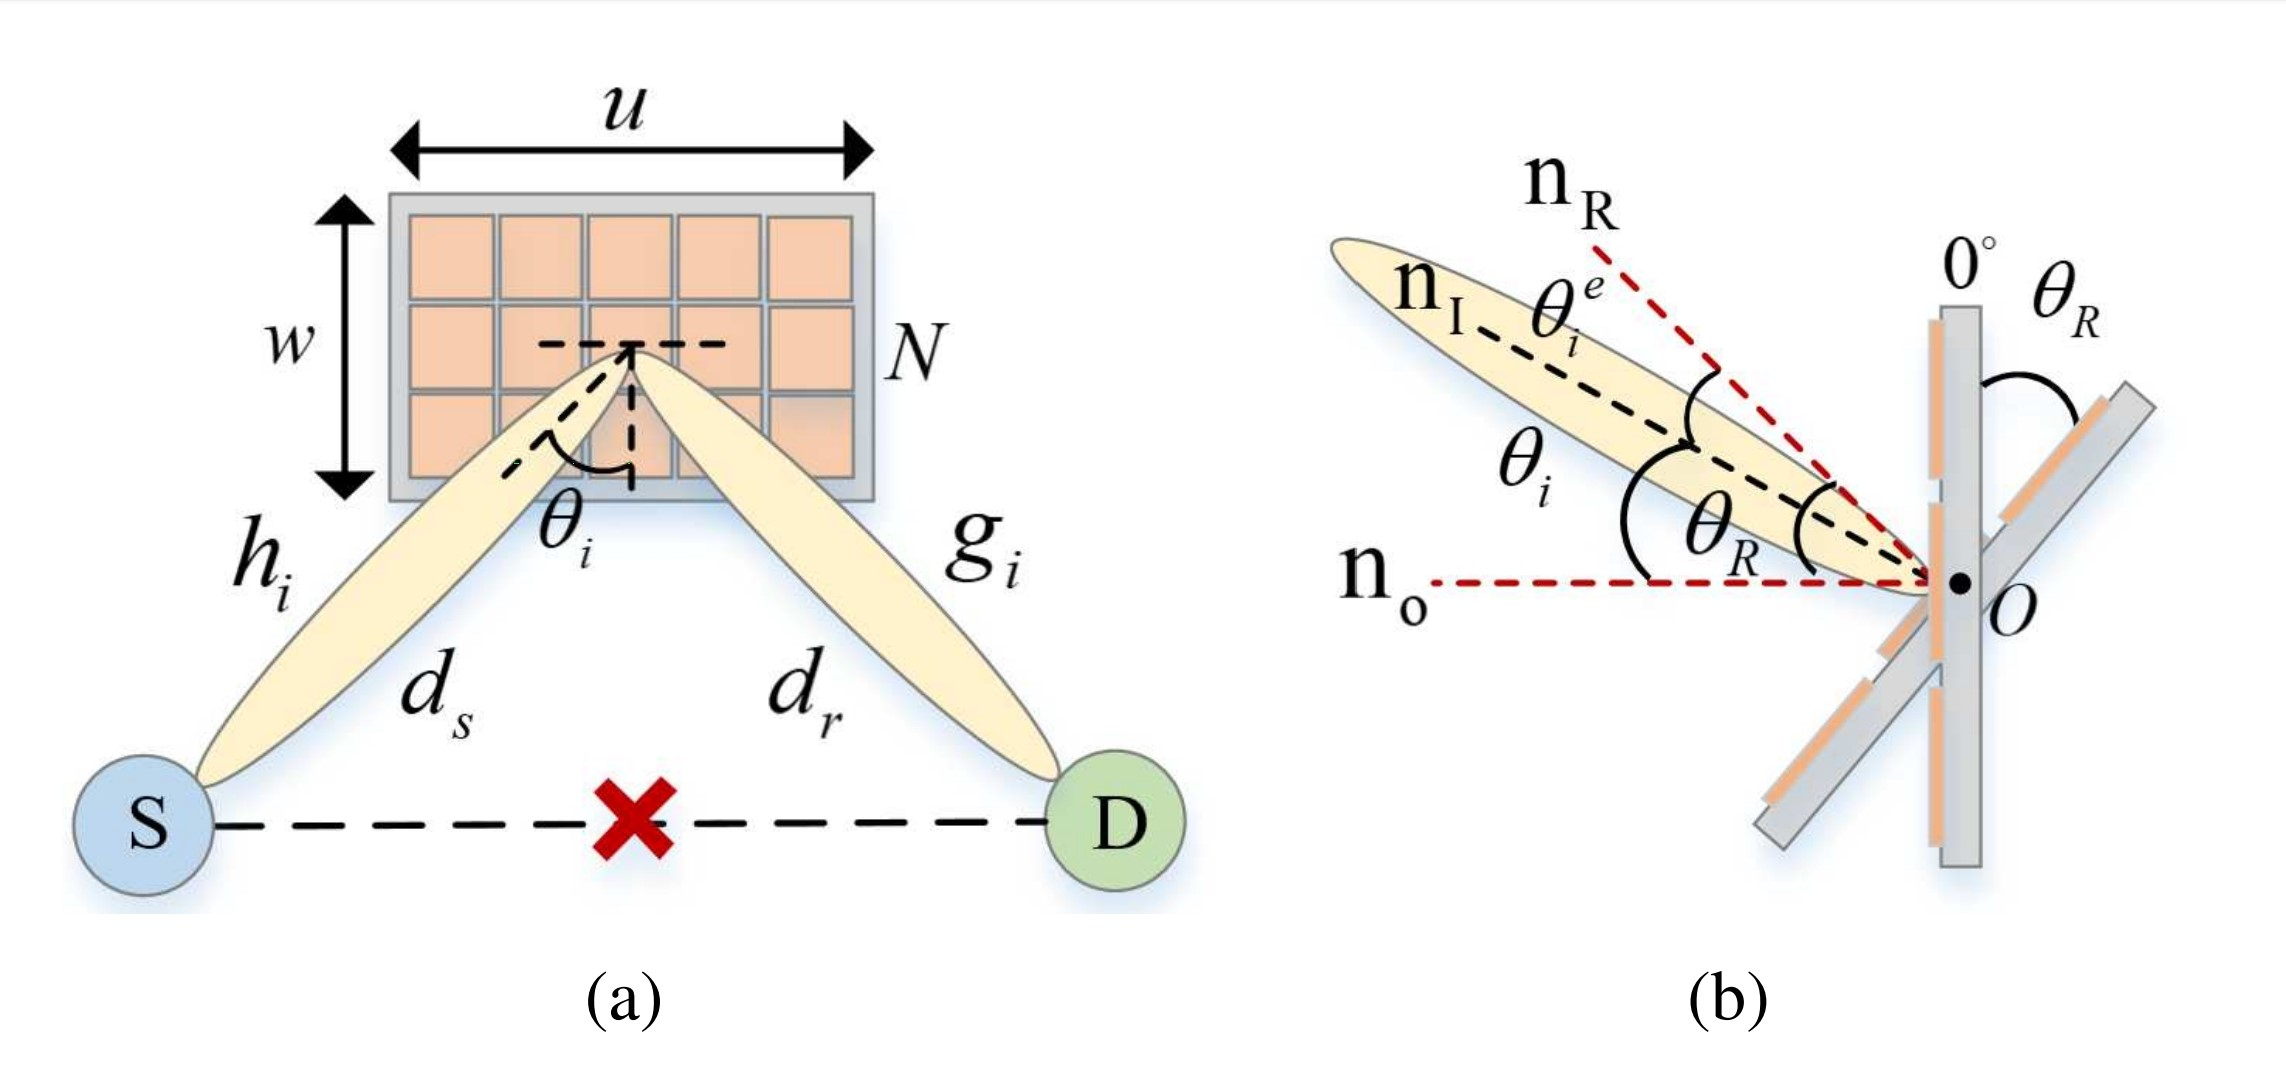
\includegraphics[scale = 0.125]{figures/system_model.jpg}
        \caption{System Model, (a) an RIS-aided communication system with N elements, (b) an illustration of the rotation of RIS plane with an angle of $\theta_R$.}
        \label{fig:system_model}
    \end{figure}
    \begin{enumerate}
        \item Here, we consider the far-field transmission for the transceivers, which means $d_s, d_r \geq \dfrac{2(\text{max}\{u,w\})^2}{\lambda}$ where, $\lambda$ is the wavelength.
        \item The angle of incidence is denoted as $\theta_i = \langle n_O, n_I\rangle$ and the angle of rotation as $\theta_R = \langle n_O, n_R\rangle$.
    \end{enumerate}
\end{frame}
\begin{frame}
\frametitle{System Model}
    \begin{block}{(A) Channel Model}
      \begin{enumerate}
        \item The realistic large-scale path loss model used in the far-field is: 
        \begin{align}
            P_l(d_s,d_r,\theta_i^e) &= \frac{G_s G_r}{(4\pi)^2}\left(\frac{u w}{d_s d_r}\right)^2\cos(\theta_i^e)
        \end{align}
        where, $G_s$ and $G_r$ are the antenna gains of transmitter and receiver, respectively. Also,  $\theta_i^e = |\theta_i - \theta_R|$
        \item The amplitudes of small-scale fading of TS and SR links are defined as $\alpha_i$ and $\beta_i$, where $i$ is the index of the element in the RIS. They both follow Rayleigh distribution with PDF given by:
        \begin{align}
            \mathnormal{f}_{\alpha}(\alpha) &= \left(\frac{\alpha}{\sigma^2}\right)\text{exp}\left(-\dfrac{\alpha^2}{2\sigma^2}\right)
        \end{align}
        where, $\sigma$ represents the fading coefficient of the channel.
      \end{enumerate}
    \end{block}
\end{frame}
\begin{frame}{System Model}
    \begin{block}{(B) Signal to Noise Ratio}
        \begin{enumerate}
            \item[1.] Assuming quasi-static Rayleigh Fading of the TS and SR links, the received signal is expressed as: 
                \begin{align}
                    y = \sqrt{P_s P_l}\left[\sum_{i=1}^{N} h_i \chi_i g_i\right]x + n_0
                \end{align}
                Here, 
                \begin{enumerate}
                    \item $x$ is transmit signal with power of $P_s$.
                    \item $\chi_i = \varrho_i(\phi_i)e^ {(j \phi_i)}$ is the reflection coefficient produced by the $i^{th}$ element.
                    \item $\varrho_i(\phi_i) = 1, \forall i = 1,2,\dots,N$ for ideal condition.
                    \item $h_i = \alpha_ie^{-j\vartheta_i}$ and $g_i = \beta_ie^{-j\varphi_i}$ are the channel gains.
                    \item $n_0$ is additive white Gaussian noise following $N(0,\sigma^2_n)$.
                \end{enumerate}
        \end{enumerate}
    \end{block}
\end{frame}
\begin{frame}{System Model}
    \begin{block}{}
        \begin{enumerate}
            \item [2.]The Signal to Noise Ratio is now given as:
                \begin{align}
                    \gamma = \frac{\left|\sum_{i=1}^{N} \alpha_i \beta_i e^{j(\phi_i - \vartheta_i - \varphi_i)}\right|^2 P_s G_s G_r (uw\times \cos{(\theta_i^e)})^2}{(4\pi \sigma_n d_s d_r)^2}
                \end{align}
                \item [3.] To obtain the maximum value of $\gamma$, the phase shift considered is $\phi_i = \vartheta_i + \varphi_i$
                \begin{align}
                    \therefore \gamma_{max} = \frac{A^2 \bar\gamma}{d_s^2 d_r^2}
                \end{align}
                where, 
                \begin{enumerate}
                    \item $A = \sum_{i=1}^{N} \alpha_i \beta_i$
                    \item Average SNR is: $\bar\gamma = \dfrac{P_s G_s G_r (u w\times \cos{(\theta_i^e)})^2}{16 \pi^2 \sigma^2_n}$,
                    here $u w \times\cos(\theta^e_i)$ represents the total effective area of the beam on the RIS from source. 
                \end{enumerate}
        \end{enumerate}
    \end{block}
\end{frame}
\begin{frame}{SNR Coverage Probability Analysis}
    Here, we first determine the distribution of $A^2$ for $N=1$ and $N\geq 1$ and the \textbf{SNR Coverage Probability} is obtained with the CDF of $A^2$
    \begin{block}{(A) SNR Coverage Probability for N = 1}
        \begin{enumerate}
            \item[1.] PDF of $\alpha\beta$:
            $\alpha$ and $\beta$ are two Independent and Identically Distributed(i.i.d.) Rayleigh Random Variables with fading coefficients \(\sigma_1\) and \(\sigma_2\). The PDF of \(\eta = \alpha\beta\) is given as:
            \begin{align}
                \mathnormal{f}_{\eta}(\eta) &= \frac{\eta}{a^2}\mathcal{K}_0\left(\frac{\eta}{a}\right)
            \end{align}
            here, $a = \sigma_1\sigma_2$ and $\mathcal{K}_0(.)$ is the zeroth order of modified Bessel function of the second kind.
            \item[2.] CDF of $\alpha\beta$: 
            \begin{align}
                \mathnormal{F}_{\eta}(\eta) = 1 - \frac{\eta}{a}\mathcal{K}_1\left(\frac{\eta}{a}\right)
            \end{align}
        \end{enumerate}
    \end{block}
\end{frame}
\begin{frame}{SNR Coverage Probability Analysis}
    \begin{block}{}
        \begin{enumerate}
            \item[] here, $\mathcal{K}_1(.)$ is the first order of modified Bessel function of the second kind.\\
            We can also obtain the CDF of $\eta^2$ by $\mathnormal{F}_{\eta^2}(\eta) = \mathnormal{F}_{\eta}(\sqrt{\eta})$ and thus, derive the SNR Coverage Probability for $N=1$.
            \item [3.] The SNR coverage probability is defined as the probability that the SNR is large than a specific threshold, which can be expressed as:
            \begin{align}
                \mathnormal{P}_{cov}(\gamma_{th}) &= \mathnormal{Pr}(\gamma \geq \gamma_{th})\\
                &= 1 - \mathnormal{Pr}(\gamma \leq \gamma_{th})\\
                &= 1 - \mathnormal{F}_{\eta^2}\left(\frac{\gamma_{th}}{\bar\gamma}d_s^2d_r^2\right)\\
                \therefore \mathnormal{P}_{cov}(\gamma_{th}) &= \frac{d_sd_r}{\sigma_1\sigma_2}\sqrt{\frac{\gamma_{th}}{\bar\gamma}}\mathcal{K}_1\left(\frac{d_sd_r}{\sigma_1\sigma_2}\sqrt{\frac{\gamma_{th}}{\bar\gamma}}\right)
            \end{align}
        \end{enumerate}
    \end{block}
\end{frame}
\begin{frame}{SNR Coverage Probability Analysis}
    \begin{block}{}
        \begin{figure}
            \centering
            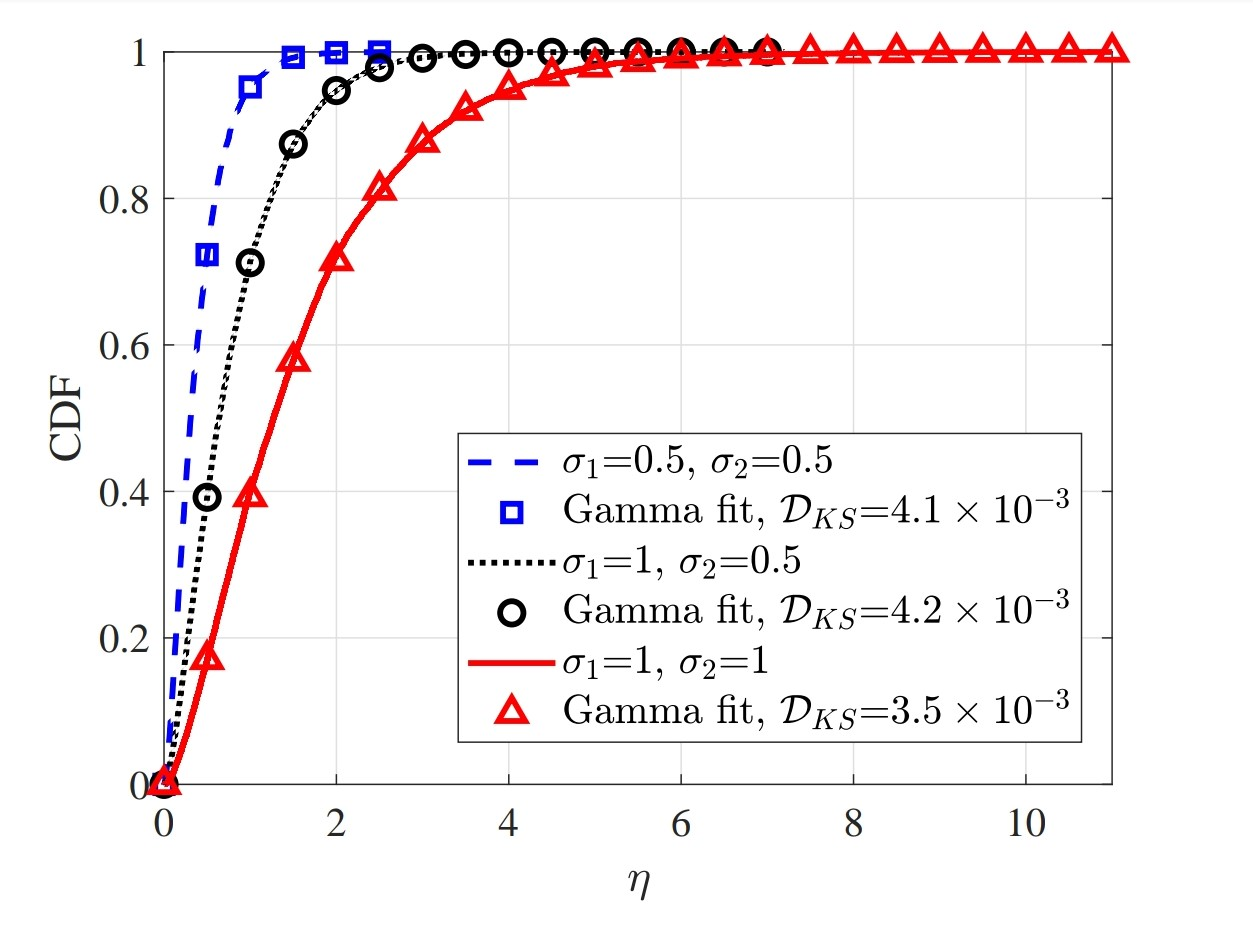
\includegraphics[scale=0.15]{figures/cdf_with_gamma_fit.jpg}
            \small{\caption{Actual CDFs of $\eta$ with Gamma fits for different fading coefficients.}}
            \label{fig:actual_cdf}
        \end{figure}
    \end{block}
    \begin{block}{(B) Approximating SNR Coverage Probability for Arbitrary N}
        The distribution of $\eta$ is in accordance to $K$-distribution $K(b, \nu)$ with $b = a = \sigma_1\sigma_2$ and $\nu = 0$. The $K$-distribution is complex and intractable. So, we use a Gamma distribution to approximate it.
    \end{block}
\end{frame}
\begin{frame}{SNR Coverage Probability Analysis}
    \begin{block}{}
        \begin{enumerate}
            \small{
            \item [1.]The distribution of $\eta$ can be approximated as Gamma distribution:
            \begin{align}
                    \eta &\sim \mathnormal{Ga}\left(\frac{\pi^2}{16 - \pi^2},\frac{16 - \pi^2}{2\pi}\sigma_1\sigma_2\right)
            \end{align}
            where,
            \begin{enumerate}
                \item $\mathnormal{Ga}(k, \theta)$ represents Gamma distribution,
                \item $\mathnormal{k} = \dfrac{\pi^2}{16 - \pi^2}$ is the shape parameter,
                \item $\theta = \dfrac{16 - \pi^2}{2\pi}\sigma_1\sigma_2$ is the scale parameter,
            \end{enumerate}
            \item[2.] The statistic $\mathcal{D_{\mathnormal{KS}}}$ is used to assess the accuracy of approximation as it finds the maximum divergence of 2 CDFs.
            \begin{align}
                \mathcal{D}_{\mathnormal{KS}} = \text{max}|\mathnormal{F}_{\text{approx}}(t) - \mathnormal{F}_{\text{actual}}(t)|
            \end{align}
            \item[3.]The Gamma function is denoted as $\Gamma(.).$} and it is highly accurate as the magnitude of $\mathcal{D}_{\mathnormal{KS}}$ is around $10^{-3}$.
        \end{enumerate}
    \end{block}
\end{frame}
\begin{frame}{SNR Coverage Probability Analysis}
    \begin{block}{}
        \begin{figure}
            \centering
            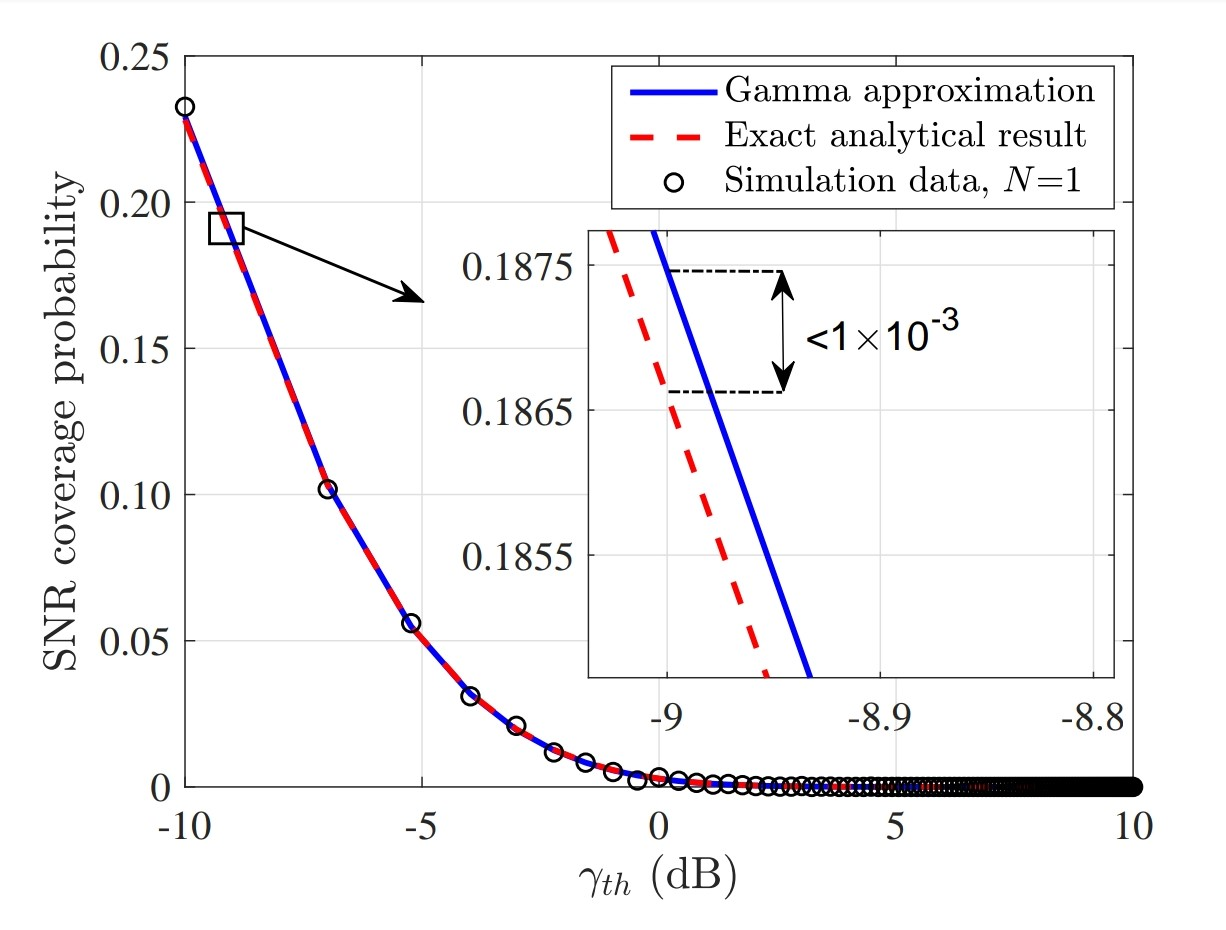
\includegraphics[scale = 0.1]{figures/result_gamma_approx_sim_with_exact_analysis.jpg}
            \caption{Results of the exact analysis, Gamma approximation, and simulation}
            \label{fig:exact_analysis}
            \centering
            \includegraphics[scale = 0.135]{figures/Gamma_vs_clt.png}
            \caption{Comparison of proposed Gamma and CLT-based Gaussian fitting}
            \label{fig:Gamma_vs_clt}
        \end{figure}
    \end{block}
\end{frame}
\begin{frame}{SNR Coverage Probability Analysis}
    \begin{block}{}
        \begin{enumerate}
            \item [4.]\small{Now, for $\mathnormal{N}$ elements in the RIS, $\mathnormal{A} \sim \mathnormal{Ga(Nk,\theta)}$.
            For $A^2$ a generalized gamma distribution is obtained with the parameters $\mathnormal{p} = 1$, $\mathnormal{d} = \dfrac{\mathnormal{Nk}}{2}$ and $\mathnormal{q} = \theta^2$ and the CDF is expressed as:}
            \begin{align}
                \mathnormal{F_{A^2}}\left(z,\frac{1}{2},\frac{\mathnormal{Nk}}{2},\theta^2\right) &= \frac{\zeta(\mathnormal{Nk},\frac{\sqrt{z}}{\theta})}{\Gamma(\mathnormal{Nk})}
            \end{align}
            here $\zeta(.,.)$ denotes lower incomplete gamma function.
            \item [5.]For arbitrary N, given the threshold $\gamma_{th}$, the general form of SNR coverage probability is expressed as:
            \begin{align}
                \mathnormal{P}_{cov}(\gamma_{th}) &= \frac{\Gamma(\mathnormal{Nk,s})}{\Gamma(\mathnormal{Nk})}
            \end{align}
            here, $s = \frac{d_sd_r}{\theta}\left(\frac{\gamma_{th}}{\bar\gamma}\right)^{\frac{1}{2}}$ and $\Gamma(.,.)$ is upper incomplete gamma function.\\
            Also, $\zeta(\mathnormal{Nk,s}) = \Gamma(\mathnormal{Nk}) - \Gamma(\mathnormal{Nk,s})$
        \end{enumerate}
    \end{block}
\end{frame}
\begin{frame}{SNR Coverage Probability Analysis}
    \begin{block}{}
        \begin{figure}
            \centering
            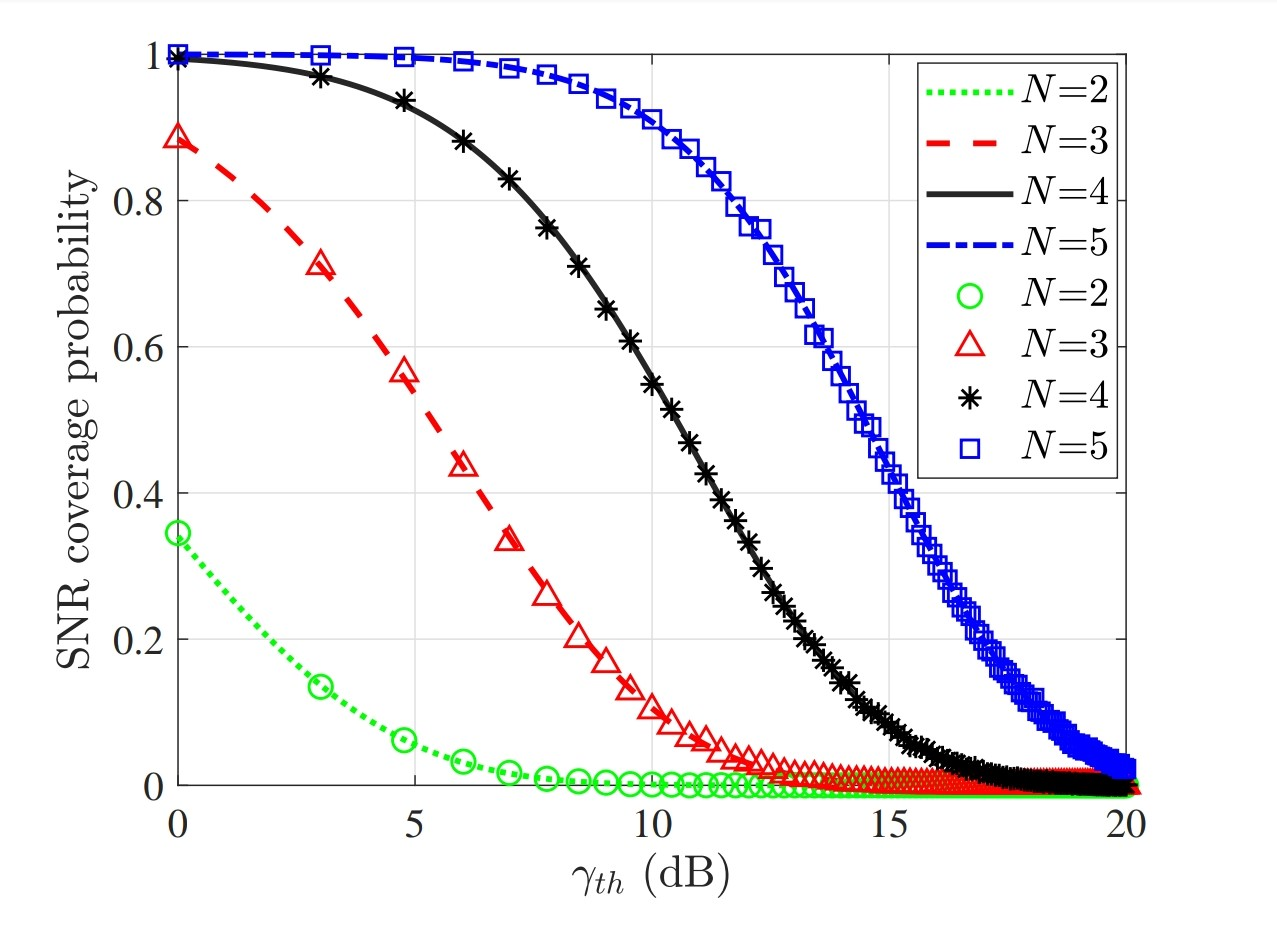
\includegraphics[scale = 0.11]{figures/gamma_sim_approx_different_N.jpg}
            \caption{Results of Gamma approximations (lines) and simulations (markers).}
            \label{fig:gamma_sim_approx_different_N}
        \end{figure}
    \end{block}    
    \begin{block}{(C) Optimal number of elements of RIS}
        \small{For infinite N, $P_{cov}=1$, but we need to have a optimal(minimum) number of RIS elements.
        \begin{align}
            \mathnormal{N}^* = min\left\{N|\Gamma(\mathnormal{Nk,s}) = \Gamma(\mathnormal{Nk})\right\},
        \end{align}
        where $\mathnormal{N^*}$ is optimal number of RIS elements and $\mathnormal{N} \in \mathbb{N}$}
    \end{block}
\end{frame}
\begin{frame}{Simulation Results}
    \small{It is seen that both the exact result and Gamma approximation are perfectly consistent with the simulation result.}
    \begin{figure}
        \centering
        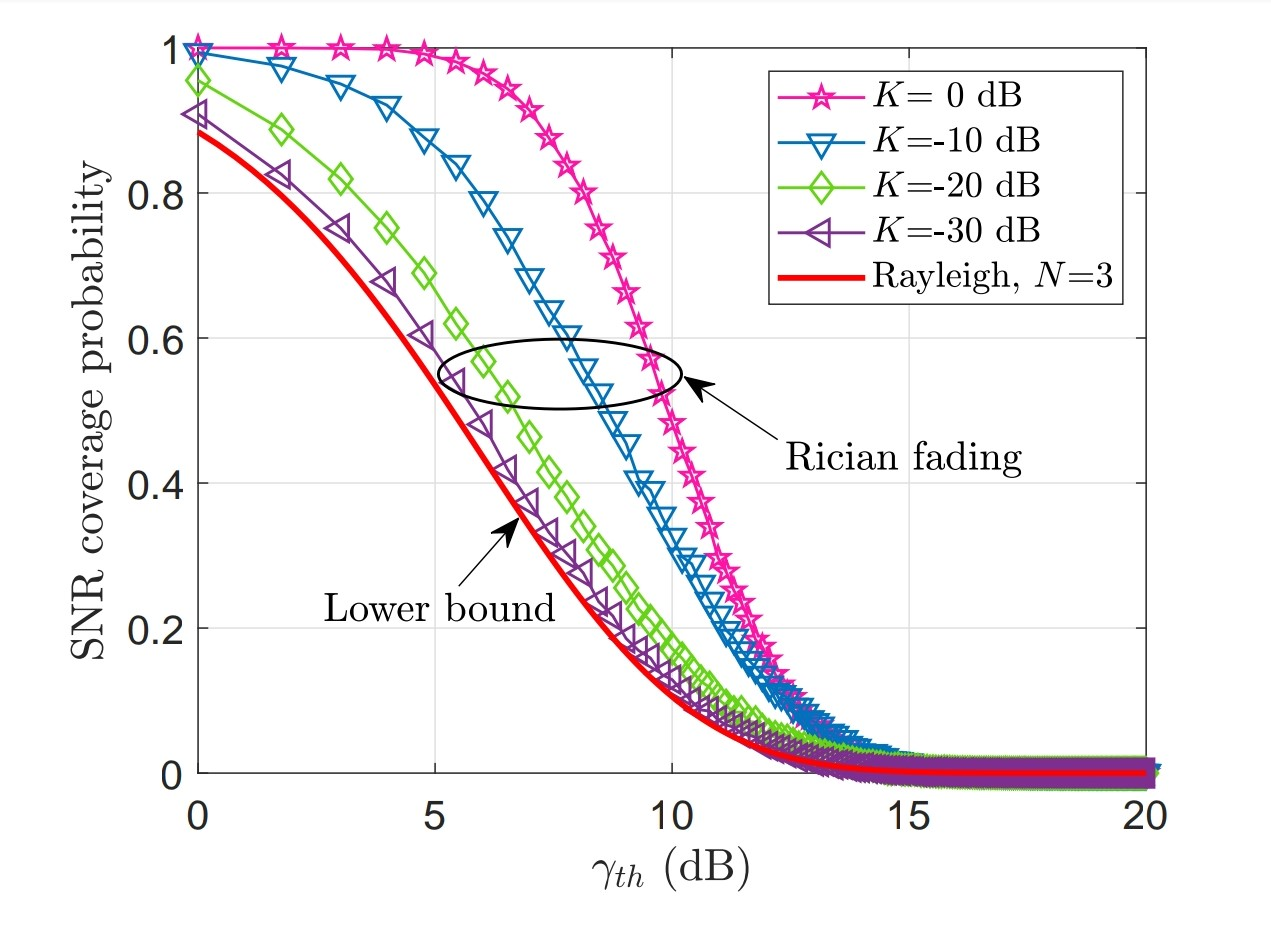
\includegraphics[scale = 0.108]{figures/rayleigh_vs_rician.jpg}
        \caption{SNR coverage probability under Rayleigh vs. Rician fading.}
        \label{fig:rayleigh_vs_rician}
        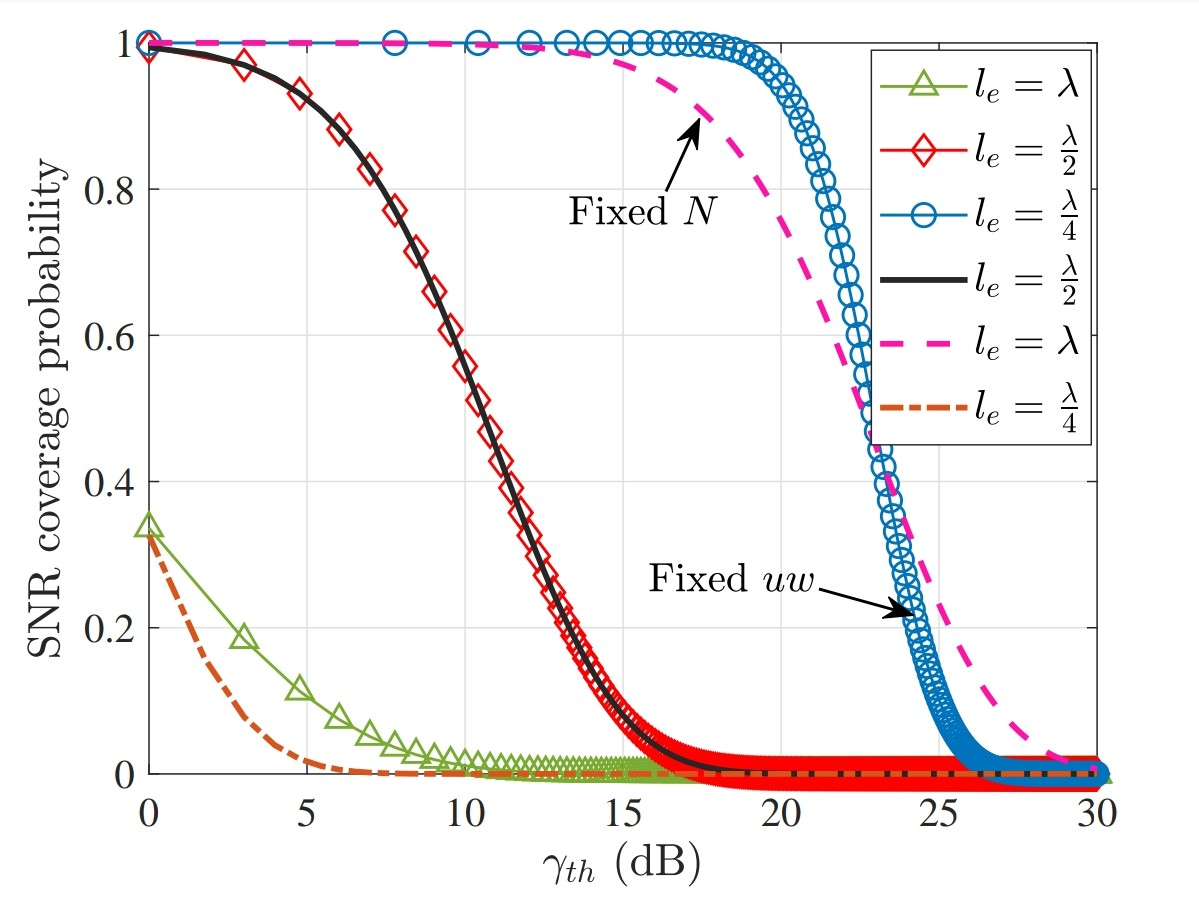
\includegraphics[scale = 0.11]{figures/SNR_vs_elementSize.jpg}
        \caption{SNR coverage probability vs. different sizes of elements.}
    \end{figure}
\end{frame}
\begin{frame}{Simulation Results}
    \begin{figure}
        \centering
        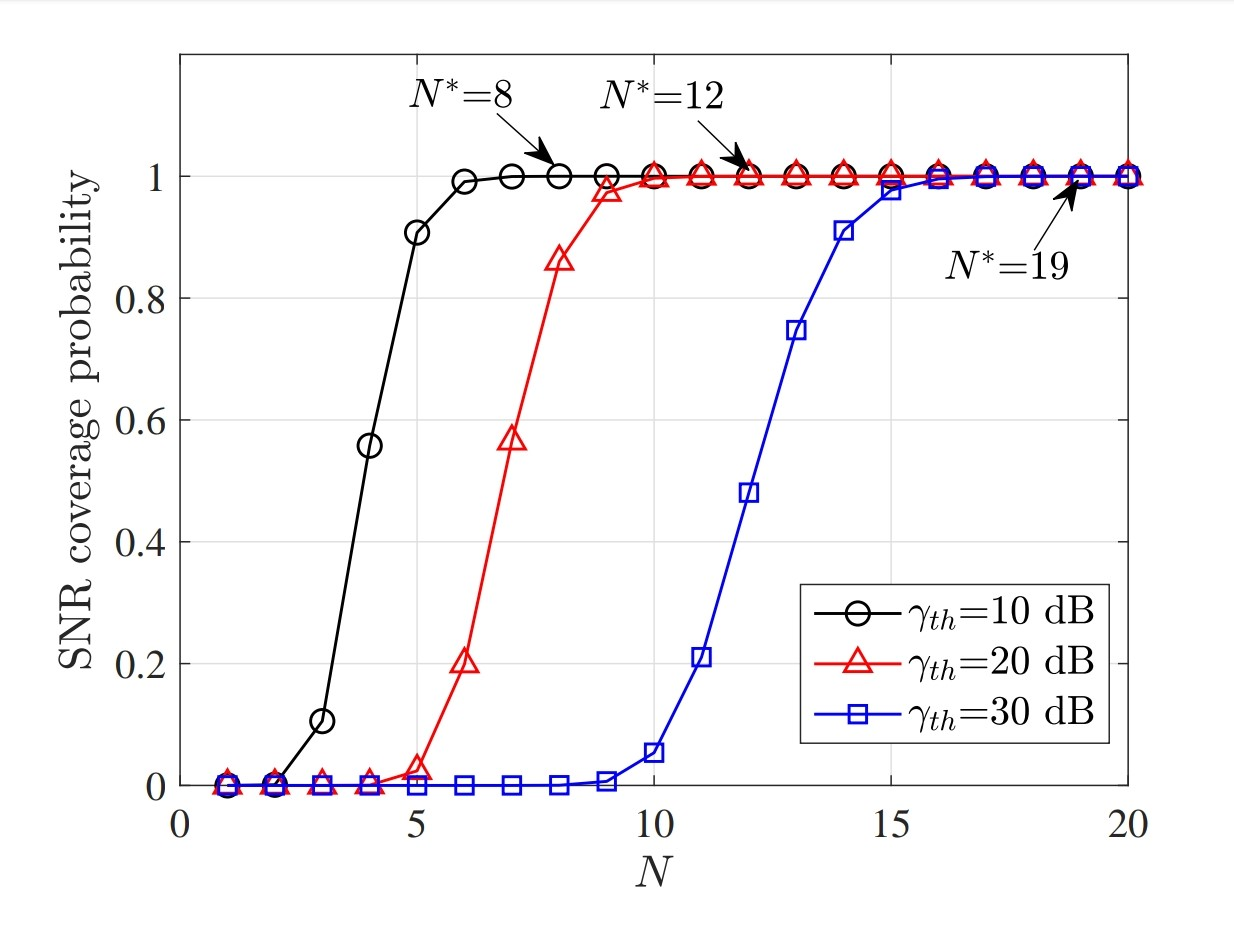
\includegraphics[scale = 0.12]{figures/SNR_cov_prob_vs_N.jpg}
        \caption{SNR coverage probability vs. N for different SNR thresholds.}
        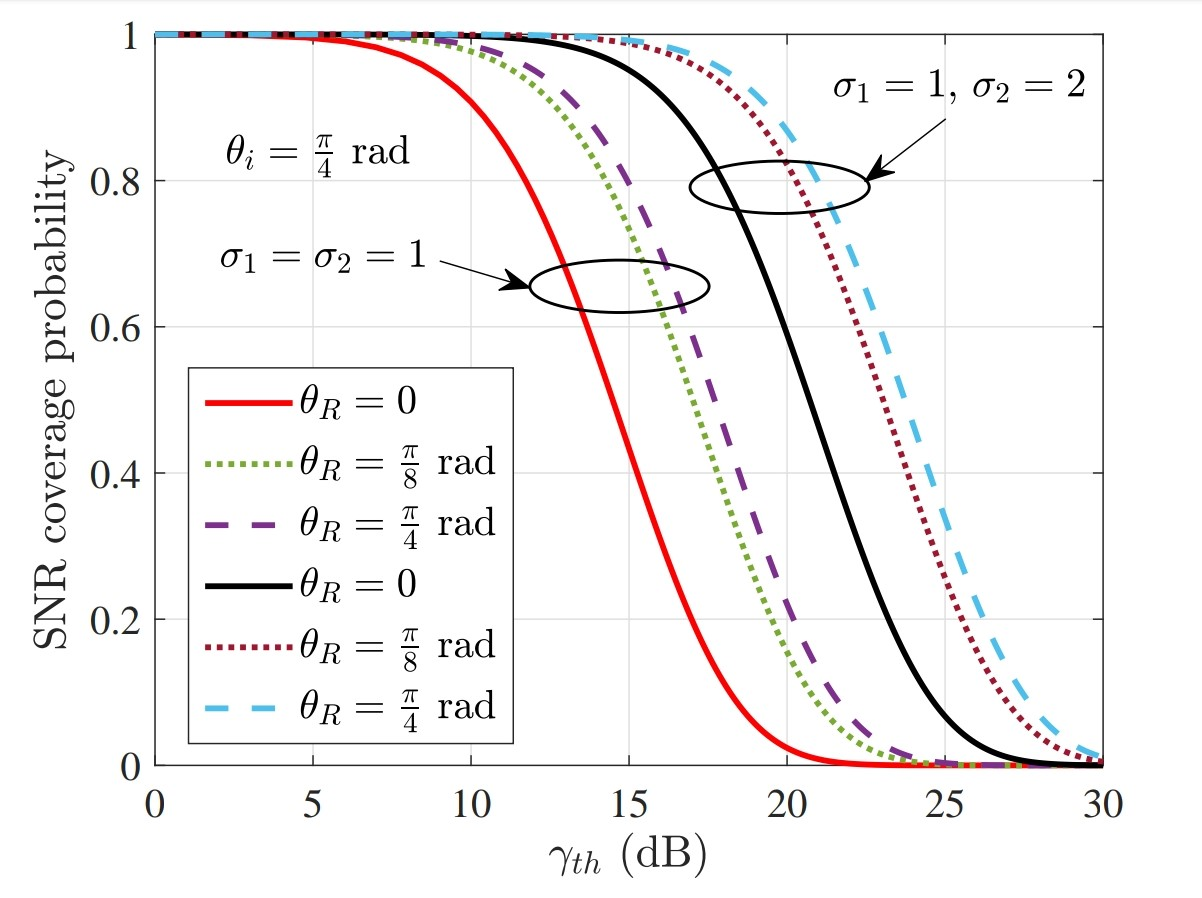
\includegraphics[scale = 0.125]{figures/SNR_vs_fadingCoeff_incidentAngle.jpg}
        \caption{SNR coverage probability vs. fading coefficients and incident angles.}
    \end{figure}
\end{frame}
\end{document}